
\documentclass[final]{beamer}

\usepackage[scale=1.24, orientation=portrait]{beamerposter} % Use the beamerposter package for laying out the poster
\usepackage{makecell}
\usetheme{confposter} % Use the confposter theme supplied with this template

\setbeamercolor{block title}{fg=ngreen,bg=white} % Colors of the block titles
\setbeamercolor{block body}{fg=black,bg=white} % Colors of the body of blocks
\setbeamercolor{block alerted title}{fg=white,bg=dblue!70} % Colors of the highlighted block titles
\setbeamercolor{block alerted body}{fg=black,bg=dblue!10} % Colors of the body of highlighted blocks
% Many more colors are available for use in beamerthemeconfposter.sty

%-----------------------------------------------------------
% Define the column widths and overall poster size
% To set effective sepwid, onecolwid and twocolwid values, first choose how many columns you want and how much separation you want between columns
% In this template, the separation width chosen is 0.024 of the paper width and a 4-column layout
% onecolwid should therefore be (1-(# of columns+1)*sepwid)/# of columns e.g. (1-(4+1)*0.024)/4 = 0.22
% Set twocolwid to be (2*onecolwid)+sepwid = 0.464
% Set threecolwid to be (3*onecolwid)+2*sepwid = 0.708

\newlength{\sepwid}
\newlength{\onecolwid}
\newlength{\twocolwid}
%\newlength{\threecolwid}
%\setlength{\paperwidth}{48in} % A0 width: 46.8in
%\setlength{\paperheight}{36in} % A0 height: 33.1in
\setlength{\paperheight}{48in} % A0 width: 46.8in
\setlength{\paperwidth}{36in} % A0 height: 33.1in
\setlength{\sepwid}{0.024\paperwidth} % Separation width (white space) between columns
\setlength{\onecolwid}{0.5\textwidth} % Width of one column
\setlength{\twocolwid}{2\onecolwid} % Width of two columns
%\setlength{\threecolwid}{3\paperwidth} % Width of three columns
\setlength{\topmargin}{-0.5in} % Reduce the top margin size
%-----------------------------------------------------------

\newcommand{\fatskip}{\vspace{3cm}}

\usepackage{graphicx}  % Required for including images

\usepackage{booktabs} % Top and bottom rules for tables

%----------------------------------------------------------------------------------------
%	TITLE SECTION 
%----------------------------------------------------------------------------------------

\title{Guitar Improvisations with Hexaphonic Multieffect (GIHME) Dataset and Practice Analysis} % Poster title

%\author{matematika.pl} % Author(s)

\author{Loïc Reboursière%\thanks{These authors contributed equally to this work}
\and
Thierry Dutoit%\textsuperscript{$\star$}
\and
Vincent Tiffon}

%----------------------------------------------------------------------------------------
\begin{document}

\addtobeamertemplate{block end}{}{\vspace*{2ex}} % White space under blocks
\addtobeamertemplate{block alerted end}{}{\vspace*{2ex}} % White space under highlighted (alert) blocks

\setlength{\belowcaptionskip}{2ex} % White space under figures
\setlength\belowdisplayshortskip{2ex} % White space under equations

\begin{frame}[t] % The whole poster is enclosed in one beamer frame

\begin{columns}[t] % The whole poster consists of three major columns, the second of which is split into two columns twice - the [t] option aligns each column's content to the top

\begin{column}{\sepwid}\end{column} % Empty spacer column

\begin{column}{\onecolwid} % The first column

%----------------------------------------------------------------------------------------
%	OVERVIEW
%----------------------------------------------------------------------------------------

\begin{alertblock}{Overview}

%We present a database of emotional speech intended to be open-sourced and used for synthesis and generation purpose. It contains data for male and female actors in English and a male actor in French. The database covers 5 emotion classes so it could be suitable to build synthesis and voice transformation systems with the potential to control the emotional dimension in a continuous way.\\
%We then present three experiments (emotional voice conversion, categorical emotional TTS, and control of emotional intensity in TTS)  and their results.


\begin{itemize}
    \item Dataset for hexaphonic guitar practice (i.e with a hexaphonic multieffect) analysis as well as MIR-related tasks
    
    \item Contains synchronized video, audio, data and transcribed interview for each improvisation recording
    
    \item Annotated data include : picth, fret, playing techniques, extended playing techniques, improvisation structure and duration, tuning and used audio effects and presets
    
    \item Open-source : \url{https://github.com/numediart/GIHME}
    
\end{itemize}



\end{alertblock}

%----------------------------------------------------------------------------------------
%	QUICK REVISION
%----------------------------------------------------------------------------------------

\begin{block}{Experiments}

%\textbf{Forms of Quadratic Function}

\begin{itemize}
    \item Two scenarios (see Table 1 and 2) were part of the recordings of the experiment. They were preceeded by a "discovery" scenario where the researcher help setting up the effects;
    \item Each sub-scenario was divided in test, improvisation recording and interview parts. These three steps could be repeated.
\end{itemize}

\\ 
\begin{table}
  
  \label{tab:scenario1}
  \begin{tabular}{ccc}
    \toprule
    Name & Strings with effects & Strings with no effect\\
    \midrule
    1\_1 & E-A-D & G-B-e\\
    1\_2 & G-B-e& E-A-D\\
    1\_3 & E-D-B & A-G-e\\
    1\_4 & A-G-e& E-D-B\\
    1\_5 & \multicolumn{2}{c}{\makecell{Distribution chosen by the guitarist}}  \\
  \bottomrule
\end{tabular}
	\caption{Scenario 1 : modification of strings allocation for chosen audio effects.}%\tablefootnote{The standard tuning of a six-string guitar is E-A-D-G-B-e, the \textbf{E} string being the 6\textsuperscript{th} string and the \textbf{e} string, the 1\textsuperscript{st} string.}.}
\end{table}
\\ \newline
\begin{table}
  
  \label{tab:scenario2}
  \begin{tabular}{cc}
    \toprule
    Name & Bypass controls mapping\\
    \midrule
    2\_1 & \makecell{1 button controls the bypass of 1 hexaphonic & effect on all strings}\\
    2\_2 & \makecell{1 button controls the bypass of the effects & applied on 1 string} \\
    2\_3 & \makecell{1 bank per effect and 1 button per string}\\
    2\_4 & \makecell{1 bank per string and 1 button per effect}\\
    2\_5 & \makecell{Distribution (2\_3 or 2\_4) chosen by the guitarist and \\ definition of recallable presets}  \\
  \bottomrule
\end{tabular}
	\caption{Scenario 2 : control of global and individual audio effects bypass.}

\end{table}

%\begin{table}[]
%\begin{tabular}{|p{0.3\onecolwid}|p{0.7\onecolwid}|}
%\hline
%Type of data & Audio, text and emotion category\\ \hline
%How data was acquired & Audio recorded in 1 anechoic chamber of the University of Mons and 2 %different anechoic chambers of the Northeastern University campus. \\ \hline
%Data format & Segmented in sentences, associated with transcriptions (CMU-Artic/SIWIS), %classified in emotional categories\\ \hline
%Experimental features & Recordings of sentences uttered by 2 male and 2 female speakers in 5 %different emotions, making a total of 7000 sentences\\ \hline
%Data accessibility & https://github.com/numediart/EmoV-DB \\
%\hline
%\end{tabular}
%\end{table}


%\fatskip
%\begin{table}
%\center
%\captionsetup{justification=centering}

%\begin{tabular}{|c|c|c|c|c|c|c|c|}
%\hline
%Speaker & Gender & Language & Neutral & Amused & Angry & Sleepy & Disgust\\
%\hline
%Spk-Je &  Female &English &417 &222 &523 &466 &189\\
%Spk-Bea &  Female &English &373 &309 &317 &520 &347\\
%Spk-Sa &  Male &English &493 &501 &468 &495 &497\\
%Spk-Jsh &  Male &English &302 &298 &- &263 &-\\
%Spk-No &  Male &French & 317 & - & 273 & - & -\\
%\hline

%\end{tabular}
%\caption{Gender and language of recorded sentences of/from each actor/speaker and amount of utterances segmented per speaker and per emotion. All speakers were recorded in all emotions, the - sign only signifies that the corresponding data were not segmented yet.}
%\end{table}

\end{block}

%------------------------------------------------

% \begin{figure}
% 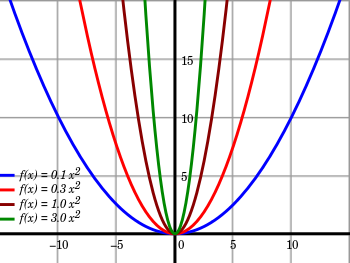
\includegraphics[width=0.8\linewidth]{1.jpg}
% \caption{Graph of $f(x)=ax^2|_{\{0.1, 0.3, 1.0, 3.0\}}$}
% \end{figure}

%----------------------------------------------------------------------------------------




%\begin{block}{Dataset}
%\end{block} 


%\begin{columns}[t,totalwidth=\twocolwid] % Split up the two columns wide column

%\begin{column}{\onecolwid}\vspace{-.6in} % The first column within column 2 (column 2.2)

%----------------------------------------------------------------------------------------
%	P
%----------------------------------------------------------------------------------------

\begin{block}{Recording setup}


%This system is built by extracting speech features with the WORLD vocoder of both source and target emotional voices, performing a Dynamic Time Warping  to align the features in time and computing a regression between the source and target features. The regression model used is a simple deep neural network (DNN) of 6 feedforward hidden layers in which each hidden layer is constituted of 1024 hyperbolic tangent units.


%\begin{figure}[h]
%\includegraphics[scale=0.7]{block_diagram_moyen}
%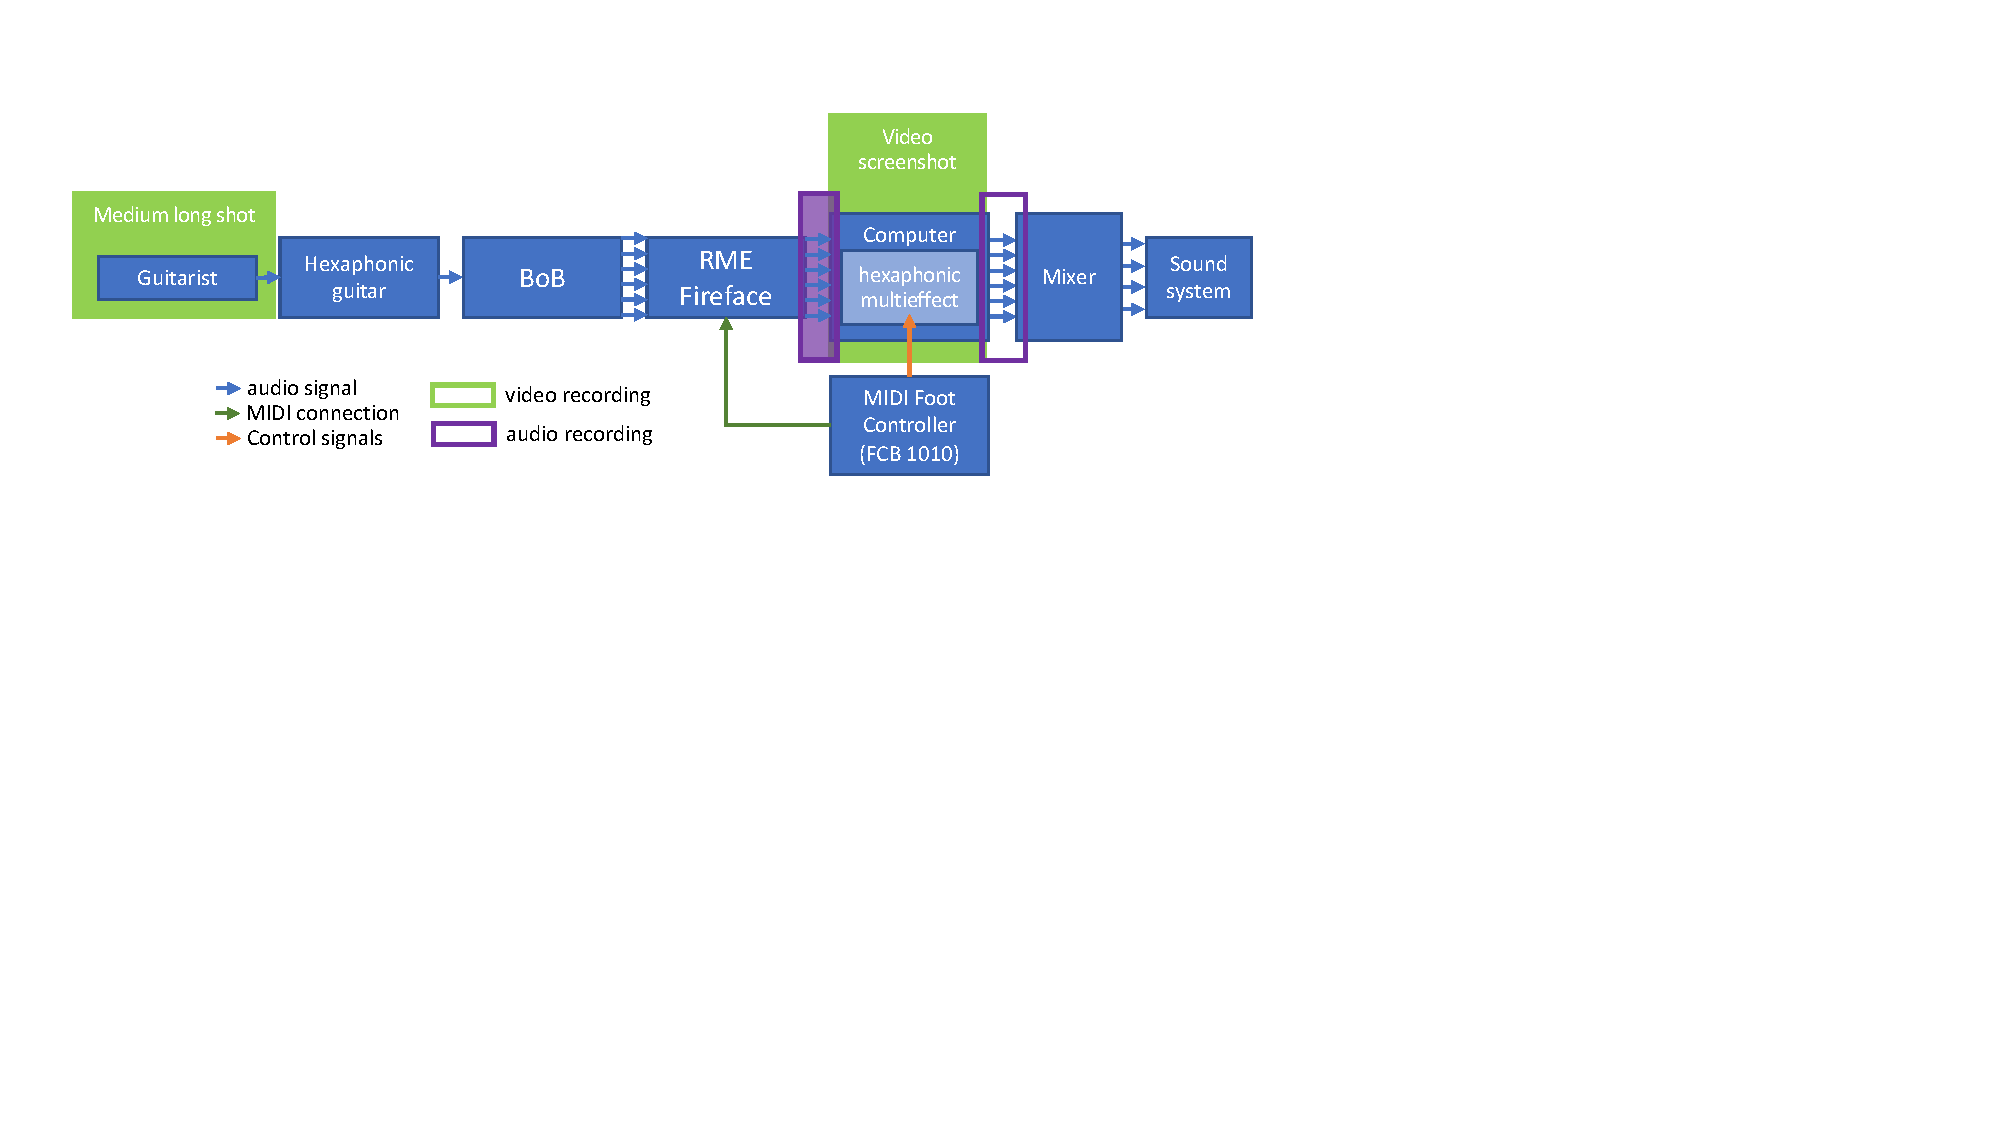
\includegraphics[width = 0.98\onecolwid]{img/experiments-recording-setup.pdf}
%\caption{Experimental audio and recording setup.}
%\label{demo}
%\end{figure}

\begin{itemize}
    \item Medium long shot of the guitarist as well as hexaphonic multieffect GUI modification were video recorded
    \item Audio recordings contain "dry" (i.e. no effect) and "wet" (i.e. with effects) hexaphonic signals as well as monophonic reduction of the wet signals
    \item Hexaphonic multieffect gathers 6 arguably "classic" audio effects for guitarists (distorsion, delay, ring modulator, flanger, tremolo and reverb) and an graphical representation of the individual bypasses as a matrix
\end{itemize}

\begin{figure}[h]
%\includegraphics[scale=0.7]{block_diagram_moyen}
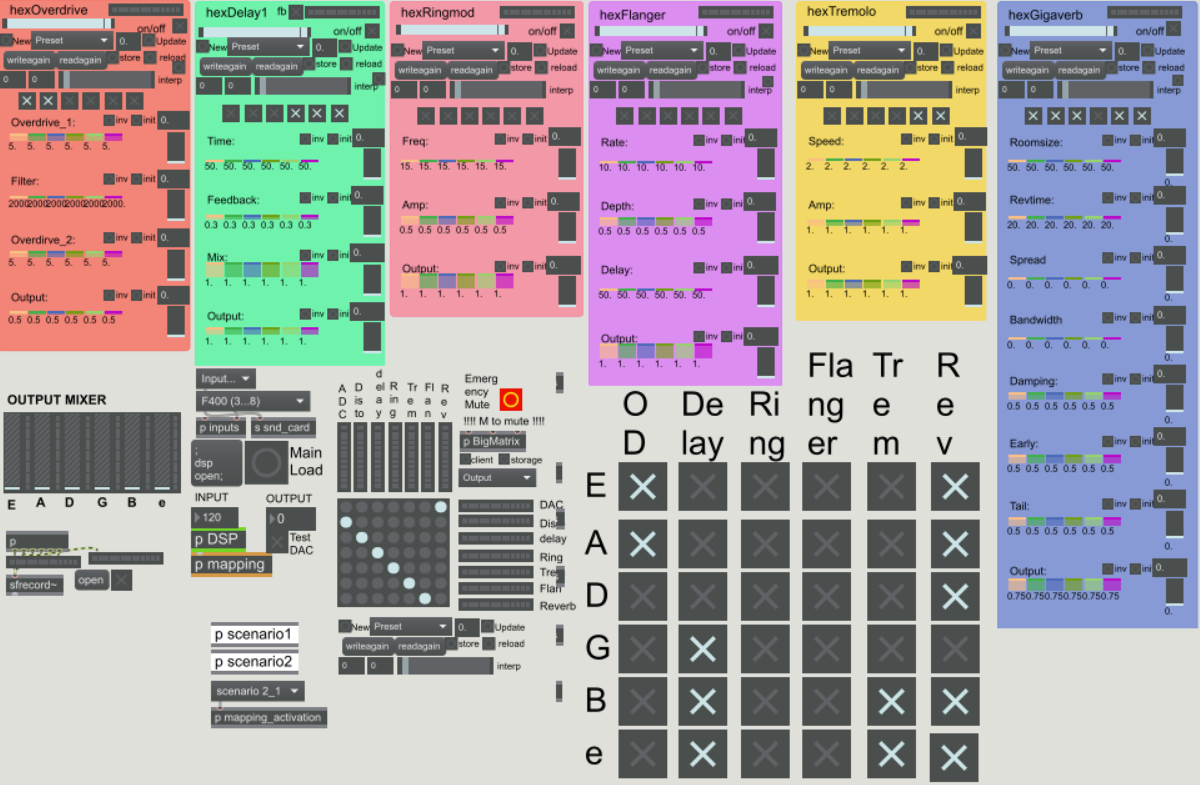
\includegraphics[width = 0.7\onecolwid]{img/191025-Patch-experience.png}
\caption{Experimental audio and recording setup.}
\label{demo}
\end{figure}

\end{block}

%----------------------------------------------------------------------------------------



%\end{column}

%\end{columns} % End of the split of column 2 - any content after this will now take up 2 columns width


%\begin{columns}[t,totalwidth=\twocolwid] % Split up the two columns wide column


\end{column} % End of the first column

\begin{column}{\sepwid}\end{column} % Empty spacer column



\begin{column}{\onecolwid} % Begin a column which is two columns wide (column 2)

%\begin{column}{\onecolwid}\vspace{-.6in} % The first column within column 2 (column 2.1)
\fatskip
\begin{block}{Dataset}

%we choose DCTTS, a system that seems to combine advantages of several systems. DCTTS models a sequence-to-sequence problem with a encoder-decoder structure along with an Attention Mechanism. Its architecture is entirely CNN-based, there is no RNN component.
%We investigate the possibility to adapt this model to have an emotional TTS. To do this, we fine-tune system to the neutral voice of one of the actresses of in our database. We then fine-tune the obtained neutral TTS model with each emotion class of the same speaker.
%The experiments performed on this dataset also assess its usability with deep learning algorithms for voice generation systems.

%Use of DCTTS (tensorflow implementation)
\begin{itemize}
    \item 5 guitarists : 
    \item 10h of musical improvisations and 4h30 of interviews
    \item Automatic (effects bypass activation), semi-automatic (pitch and fret), manual  (playing techniques and extended playing techniques) and global (tuning, improvisation structure, used effects and presets) annotations
    \item All the interviews have been transcribed
\end{itemize}


\begin{figure}[h]
%\includegraphics[scale=0.7]{block_diagram_moyen}
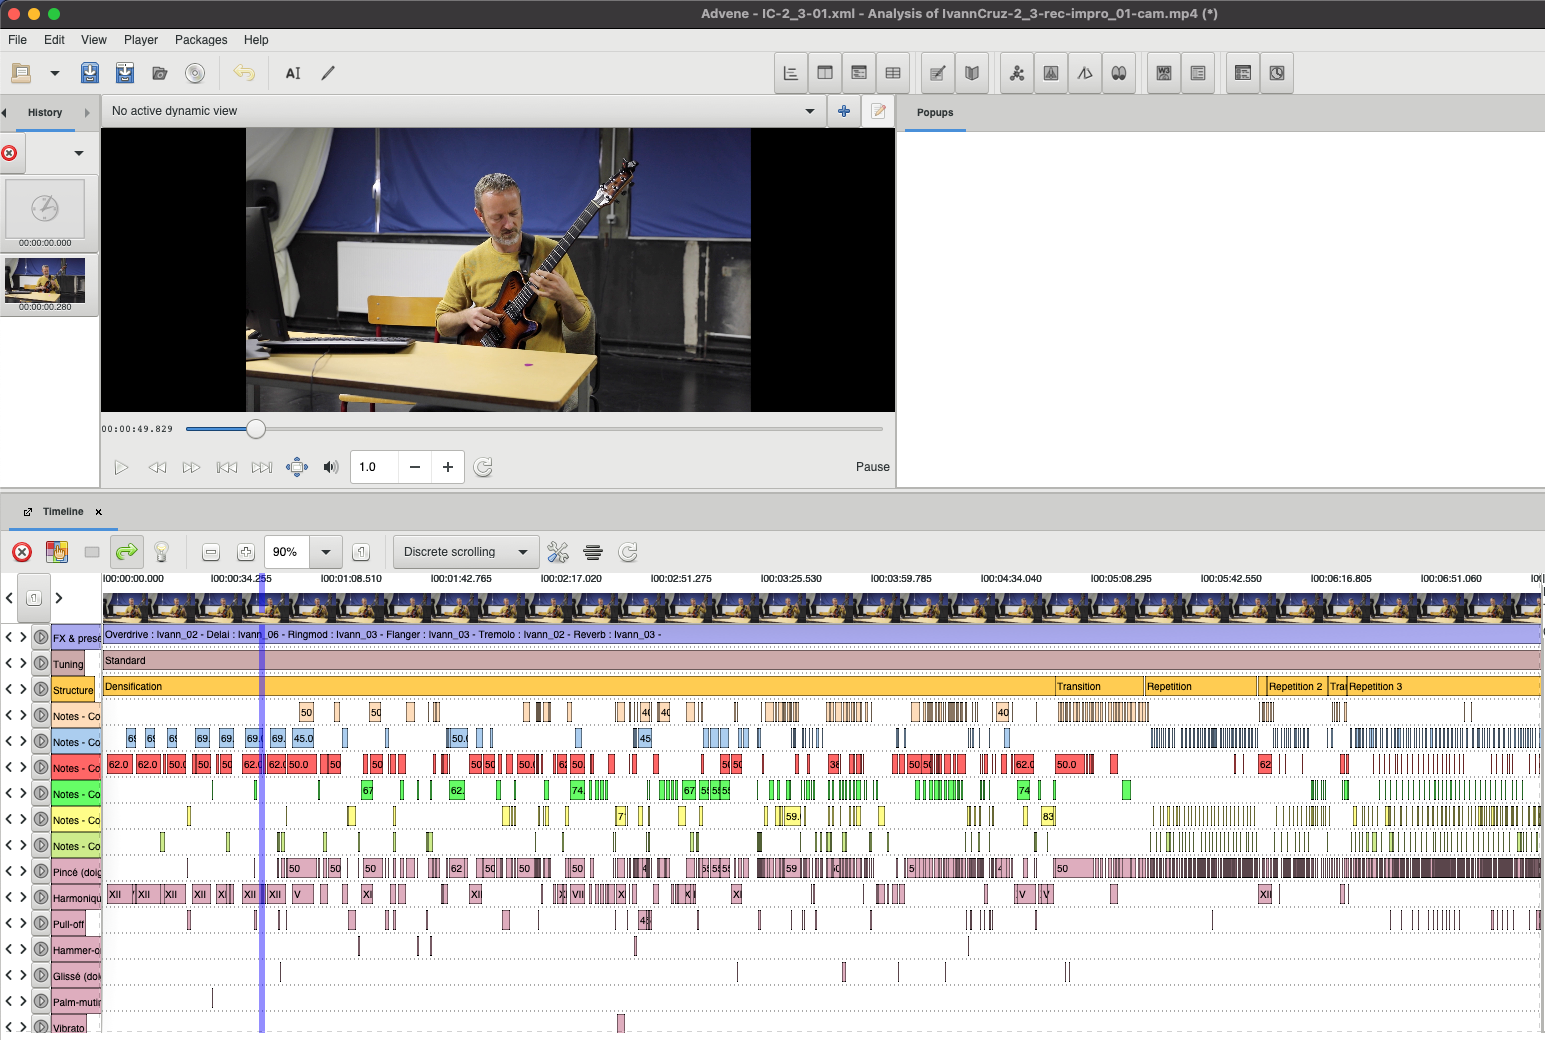
\includegraphics[width = 0.98\onecolwid]{img/IvannCruz_2_3_1_Advene.png}
\caption{GIHME annotations integration example in Advene software.}
\label{demo}
\end{figure}

\end{block}

%----------------------------------------------------------------------------------------

%\end{column} % End of column 2.1

%\begin{column}{\onecolwid}\vspace{-.6in} % The second column within column 2 (column 2.2)



%\end{column}

%\end{columns} % End of the split of column 2 - any content after this will now take up 2 columns width



%\begin{columns}[t,totalwidth=\twocolwid] % Split up the two columns wide column

%\begin{column}{\onecolwid}\vspace{-.6in} % The first column within column 2 (column 2.2)

%----------------------------------------------------------------------------------------
%	P
%----------------------------------------------------------------------------------------
\fatskip
\begin{block}{Analysis}
\begin{itemize}
    \item First analysis based on the transcriptions of the interviews.
    \item All guitarists felt, at some point, constrained by the setup or by the scenarios but eventually find ways around those constraints
    \item Despite being more "complex" the system respect the practice of the guitarist\\ 
    \begin{quote}
     It doesn't question the practice. The practice stays, it exists. However, it reconsiders it, in the sense where, as new things happen, you have to adapt. [...] It's a system that forces you to look deeply at the instrument for ways to adapt, even if it is a material that I know. (Guitarist 2, extract of post improvisation interview, scenario2\_5, pers. comm.)
    \end{quote}
    \item This system brings extensive sound possibilities and easily fits in practices that uses extremly individualisation of the strings such as classical guitar or prepared guitar practices\\ 
\begin{quote}
With a classical guitar, we work with the aim of being able to have an action as independent as possible from each finger and therefore potentially also differentiated regarding the strings. (Guitarist 4, complementary interview, pers. comm.)
\end{quote}
\end{itemize}

%multi-emotional TTS system with the possibility to control the intensity of emotional categories. We implemented a modified version of DCTTS that takes an encoding of the emotion category at the input of the decoder. During training, a simple one-hot encoding is used. But at synthesis stage, we can modify the intensity of an emotion category by inputting numbers smaller or greater than one. 
%The results sound encouraging and we are planning to do some subjective evaluations to assess the system.

    

    


\end{block}

%----------------------------------------------------------------------------------------

%\end{column} % End of column 2.1

%\begin{column}{\onecolwid}\vspace{-.6in} % The second column within column 2 (column 2.2)


%\end{column}

%\end{columns} % End of the split of column 2 - any content after this will now take up 2 columns width


%----------------------------------------------------------------------------------------
%	IMPORTANT To REMEMBER
%----------------------------------------------------------------------------------------

%\setbeamercolor{block alerted title}{fg=black,bg=norange} % Change the alert block title colors
%\setbeamercolor{block alerted body}{fg=black,bg=white} % Change the alert block body colors

\begin{alertblock}{Future Works}

\begin{itemize}
    \item Perception Tests for the last experiment
    \item Multi-speaker model (For now we use the data from only one speaker)
    \item Synthesis with non-verbal expressions
\end{itemize}

\end{alertblock} 

%----------------------------------------------------------------------------------------


%\end{column} % End of the second column

\begin{column}{\sepwid}\end{column} % Empty spacer column

%\begin{column}{\onecolwid} % The third column

%----------------------------------------------------------------------------------------
%	CONCLUSION
%----------------------------------------------------------------------------------------



%----------------------------------------------------------------------------------------
%	ACKNOWLEDGEMENTS
%----------------------------------------------------------------------------------------


%----------------------------------------------------------------------------------------

\end{column} % End of the third column

\end{columns} % End of all the columns in the poster

\end{frame} % End of the enclosing frame

\end{document}
